\paragraph{The active case.} The next step, of course, is to make the flow
actually depend on the composition. After all, compositional fields are not only
intended to indicate where material come from, but also to indicate the
properties of this material. In general, the way to achieve this is to write
material models where the density, viscosity, and other parameters depend on the
composition, taking into account what the compositional fields actually denote
(e.g., if they simply indicate the origin of material, or the concentration of
things like olivine, perovskite, \ldots). The construction of material models is
discussed in much greater detail in Section~\ref{sec:material-models}; we do not
want to revisit this issue here and instead choose -- once again -- the simplest
material model that is implemented in \aspect{}: the \texttt{simple} model.

The place where we are going to hook in a compositional dependence is the
density. In the \texttt{simple} model, the density is fundamentally described by
a material that expands linearly with the temperature; for small density
variations, this corresponds to a density model of the form
$\rho(T)=\rho_0(1-\alpha(T-T_0))$. This is, by virtue of its simplicity, the
most often considered density model. But the \texttt{simple} model also has a
hook to make the density depend on the first compositional field $c_1(\mathbf
x,t)$, yielding a dependence of the form
$\rho(T)=\rho_0(1-\alpha(T-T_0))+\gamma c_1$. Here, let us choose $\rho_0=1,
\alpha=0.01, T_0=0, \gamma=100$. The rest of our model setup will be as
in the passive case above. Because the temperature will be between zero and one,
the temperature induced density variations will be restricted to 0.01, whereas
the density variation by origin of the material is 100. This should make sure
that dense material remains at the bottom despite the fact that it is hotter
than the surrounding material.%
\footnote{The actual values do not matter as much here. They are chosen in such
a way that the system -- previously driven primarily by the velocity boundary
conditions at the top -- now also feels the impact of the density variations.
To have an effect, the buoyancy induced by the density difference between
materials must be strong enough to balance or at least approach the forces
exerted by whatever is driving the velocity at the top.}


This setup of the problem can be described using an input file that is almost
completely unchanged from the passive case. The only difference is the use of
the following section (the complete input file can be found in
\url{cookbooks/composition\_active/composition\_active.prm}:

\lstinputlisting[language=prmfile]{active.part.prm.out}

To debug the model, we will also want to visualize the density in our
graphical output files. This is done using the following addition to the
postprocessing section, using the \texttt{density} visualization plugin:
\lstinputlisting[language=prmfile]{postprocess.part.prm.out}

\begin{figure}
  \centering
  \centering
  \includegraphics[width=0.3\textwidth]{visit0007.png}
  \hfill
  \includegraphics[width=0.3\textwidth]{visit0009.png}
  \hfill
  \includegraphics[width=0.3\textwidth]{visit0008.png}
  \caption{\it Active compositional fields: Compositional field 1 at the time
    $t=0, 10, 20$. Compared to the results shown in
    Fig.~\ref{fig:compositional-passive} it is clear that the heavy material
    stays at the bottom of the domain now. The effect of the density on the
    velocity field is also clearly visible by noting that at all three times
    the spreading center at the top boundary is in exactly the same position;
    this would result in exactly the same velocity field if the density and
    temperature were constant.}
  \label{fig:composition-active-composition}
\end{figure}

\begin{figure}
  \centering
  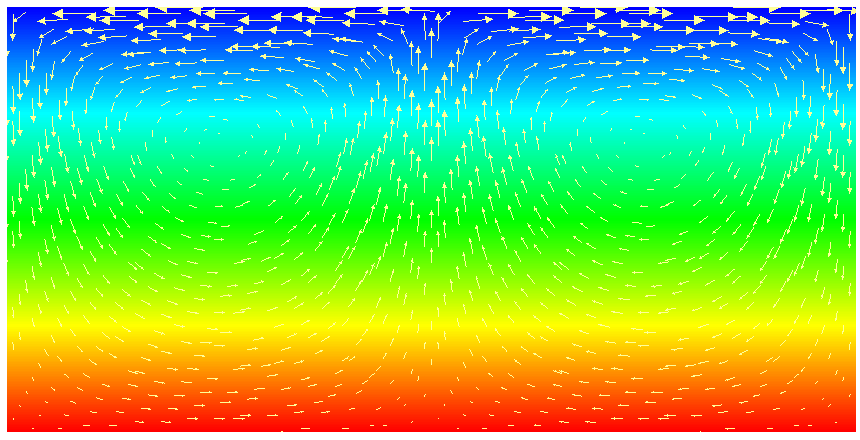
\includegraphics[width=0.3\textwidth]{visit0000.png}
  \hfill
  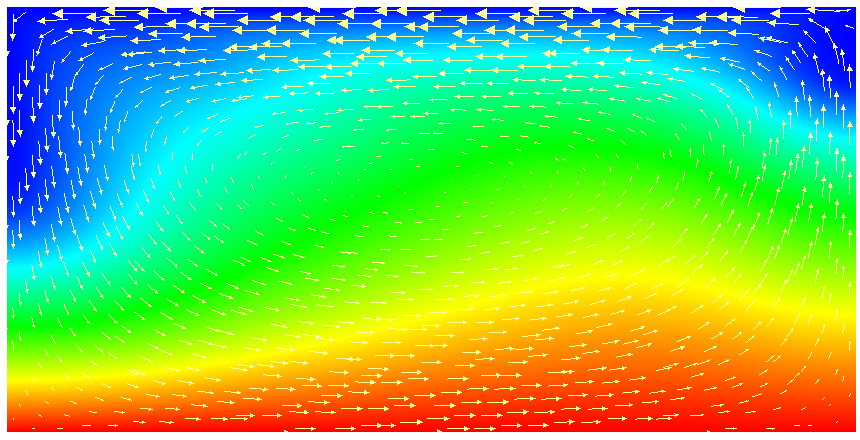
\includegraphics[width=0.3\textwidth]{visit0001.png}
  \hfill
  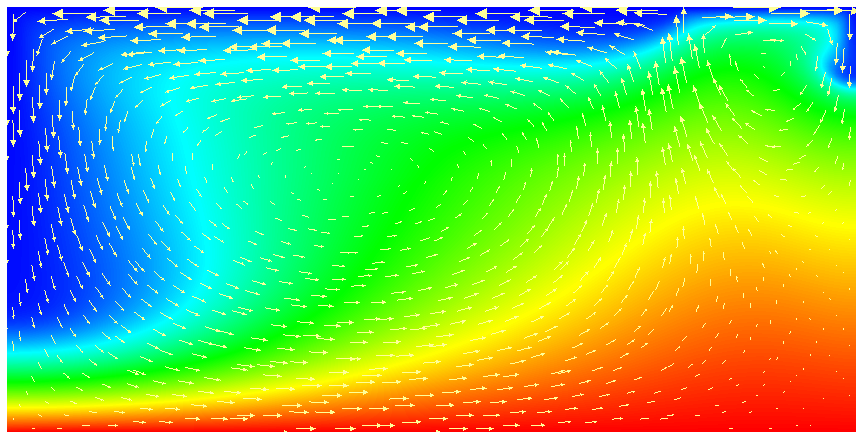
\includegraphics[width=0.3\textwidth]{visit0002.png}
  \\[6pt]
  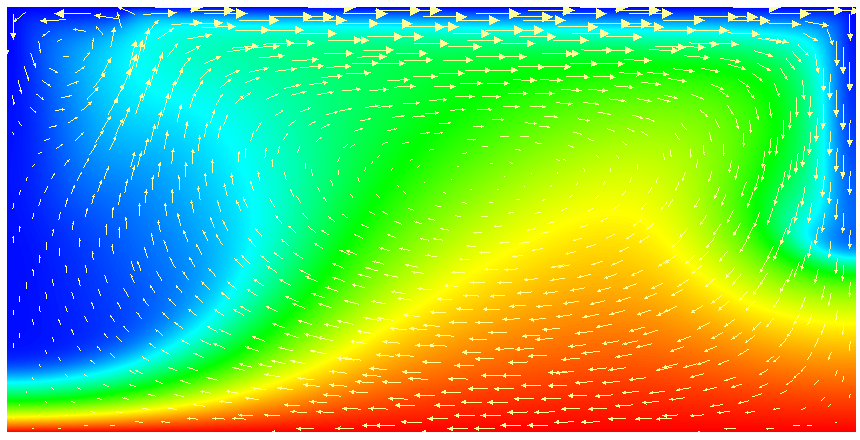
\includegraphics[width=0.3\textwidth]{visit0003.png}
  \hfill
  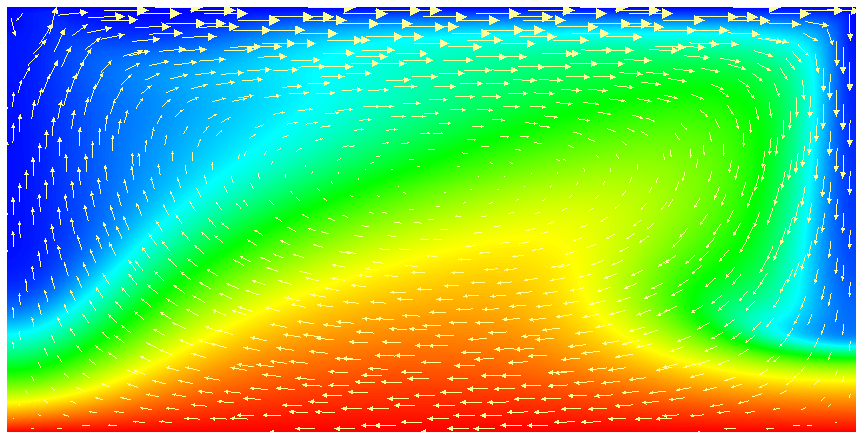
\includegraphics[width=0.3\textwidth]{visit0004.png}
  \hfill
  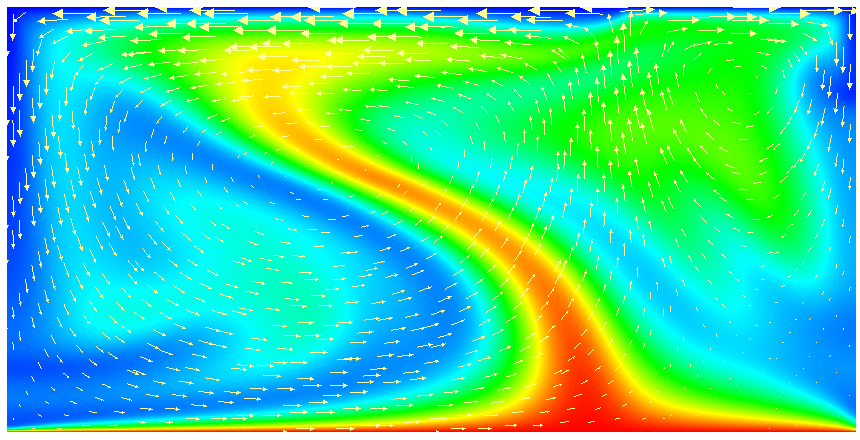
\includegraphics[width=0.3\textwidth]{visit0006.png}
  \caption{\it Active compositional fields: Temperature fields at $t=0, 2, 4, 8,
  12, 20$. The black line is the isocontour line $c_1(\mathbf x,t)=0.5$
    delineating the position of the dense material at the bottom.}
  \label{fig:composition-active-temperature}
\end{figure}

Results of this model are visualized in
Figs.~\ref{fig:composition-active-composition} and \ref{fig:composition-active-temperature}. What is visible is
that over the course of the simulation, the material that starts at the bottom
of the domain remains there. This can only happen if the circulation is
significantly affected by the high density material once the interface starts
to become non-horizontal, and this is
indeed visible in the velocity vectors. As a second consequence, if the
material at the bottom does not move away, then there needs to be a different
way for the heat provided at the bottom to get through the bottom layer:
either there must be a secondary convection system in the bottom layer, or
heat is simply conducted. The pictures in the figure seem to suggest
that the latter is the case.

It is easy, using the
outline above, to play with the various factors that drive this system, namely:
\begin{itemize}
  \item The magnitude of the velocity prescribed at the top.
  \item The magnitude of the velocities induced by thermal buoyancy, as
  resulting from the magnitude of gravity and the thermal expansion coefficient.
  \item The magnitude of the velocities induced by compositional variability, as
  described by the coefficient $\gamma$ and the magnitude of gravity.
\end{itemize}
Using the coefficients involved in these considerations, it is trivially
possible to map out the parameter space to find which of these effects is
dominant. As mentioned in discussing the values in the input file, what is
important is the \textit{relative} size of these parameters, not the fact
that currently the density in the material at the bottom is 100 times larger
than in the rest of the domain, an effect that from a physical perspective
clearly makes no sense at all.

